\documentclass[UTF8]{ctexart}
\usepackage{graphicx}
\usepackage{float}
\title{实验报告3}
\author{}
\begin{document}
\maketitle
\begin{flushleft}
\section{实验项目}
Web搜索引擎实现
\section{实验环境}
Java + eclipse + string tool suite
\section{实现要求}
\subsection{网页抓取:5+南开校内网站,10000+网页}
\subsection{文本索引:网页及其锚文本+}
\subsection{链接分析:PageRank}
\subsection{查询服务:}
\subsubsection*{site,filetype}
\subsubsection*{短语,通配}
\subsubsection*{日志}
\subsubsection*{网页快照}
\subsection{搜索主题:学院网新闻}
\subsection{作业文档:latex}
\section{实验分析}
分为以下几个步骤:
\begin{itemize}
  \item 爬虫,将每个网页的有效信息爬下来。我爬了南开大学哲学院、软件学院、经济学院、文学院、金融学院、汉语言文学院、数学院、环境科学学院、旅游学院的学院官网,由于害怕对一个网站爬太多网页会被识破被拒绝访问,我设置了一个阈值,一个学院最多爬1501个网页。
  \item 	 计算pagerank值。在上一步,对于每一个网页中爬取到的信息,用文档保存,文档中还保存了这个网页指向的网页被代表的id号。依据我的计算,所有网页(一万多个)的pr值总和为1,所以几乎所有pr值都是E-5数量级的。
  \item
      利用lucene和中文分词器IKAnalyzer生成索引,并设置查找的函数。
\end{itemize}
\section{实验效果截图}
\subsection{5+南开校内网站,10000+网页}
我爬了9个南开校内网站,10000+网页
如下图,不同的网站我存在不同的文件夹里:
\par{}
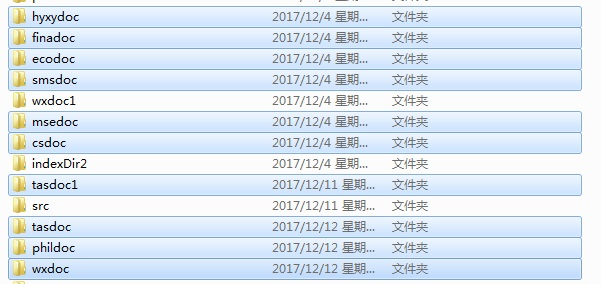
\includegraphics[width=5.00in,height=2.80in]{figure22.jpg}
\par{}
在这10000+网页中我们进行搜索
\par{}
搜索界面:
\par{}

\includegraphics[width=3.00in,height=1.50in]{figure7.jpg}
\par{}
结果界面:(其中score为\textbf{pagerank值})
\par{}
在10000+的网页里,我们搜索魏大鹏,既能读到软件学院的信息,又能读到数学学院、文学院等多个网站的新闻。
\par{}
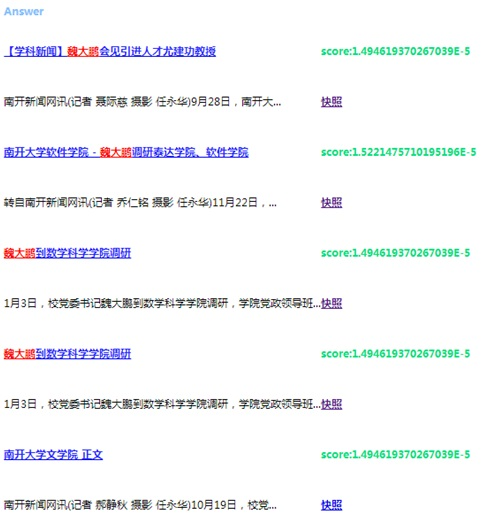
\includegraphics[width=5.00in,height=5.00in]{figure8.jpg}
\par{}
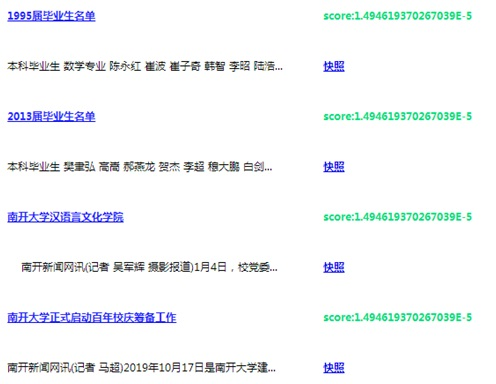
\includegraphics[width=5.00in,height=3.80in]{figure9.jpg}
\par{}
    把鼠标放在每一个标题的上面,如果点击就会进入那个页面,我们只是浮于标题之上,根据浏览器下方显示网址的网址知道是可以点击进入那个网页的:
\par{}
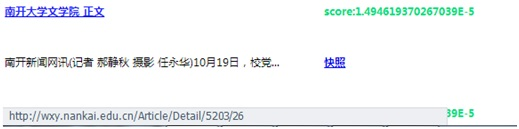
\includegraphics[width=5.00in,height=1.20in]{figure10.jpg}
\par{}
\textbf{我们测试搜索一句话:}
\par{}
"魏大鹏到数学科学学院"
\par{}
得到如下结果
\par{}
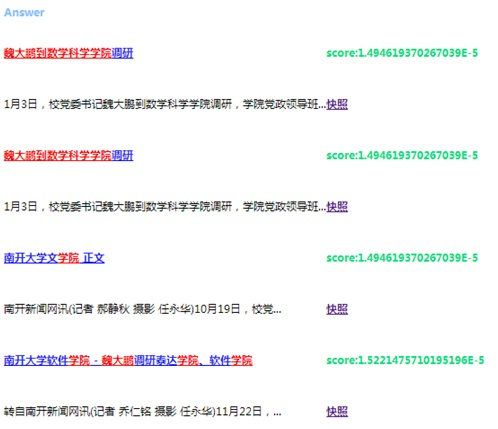
\includegraphics[width=5.00in,height=4.30in]{figure13.jpg}
\par{}
\par{}
生成的\textbf{日志}如下:
\par{}
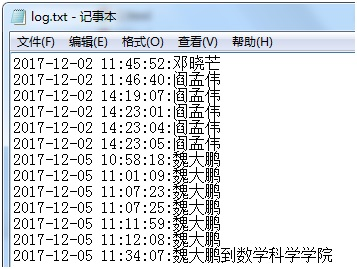
\includegraphics[width=3.50in,height=2.60in]{figure14.jpg}
\par{}
共有如下图所示数量文件,由于文件的总体积太大无法上传
\par{}
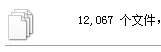
\includegraphics[width=1.00in,height=0.50in]{figure32.jpg}
\par{}
我另外写了一个小demo,里面包含了文学院的50个网页(在实际的10000+网页中,有1501个文学院的网页)
\par{}
我上传的wxdoc文件夹里
\par{}
html文件夹里存放html文件,用于快照\par{}anchor文件夹里存放锚文本\par{}url文件存放url信息\par{}其余的以数字命名的文件代表了对应url的信息。
\subsection{下图为爬虫之后存储的文件:}
\par{}
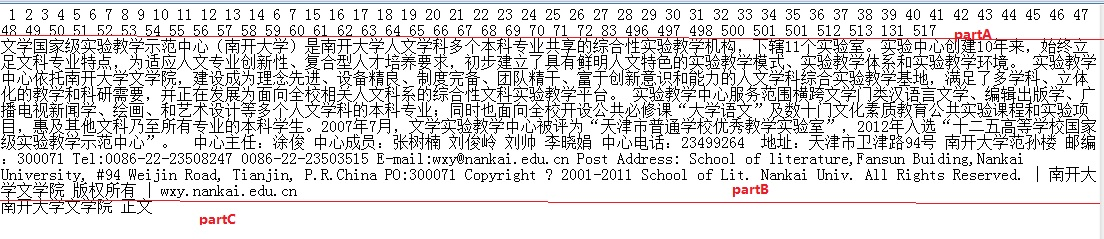
\includegraphics[width=5.00in,height=2.50in]{figure6.jpg}
\par{}
其中partA是代表它指向链接的id号
\par{}
partB代表\textbf{网页的内容}
\par{}
partC代表网页的标题
\par{}
\subsection{锚文本信息}
我上传的wxdoc和phildoc文件夹里有anchor文件夹,里面存放着相应的锚文本信息
\par{}
下图是一个文件的内容,代表指向它的锚文本内容,我们发现,指向这个url的所有锚文本都是学院首页
\par{}
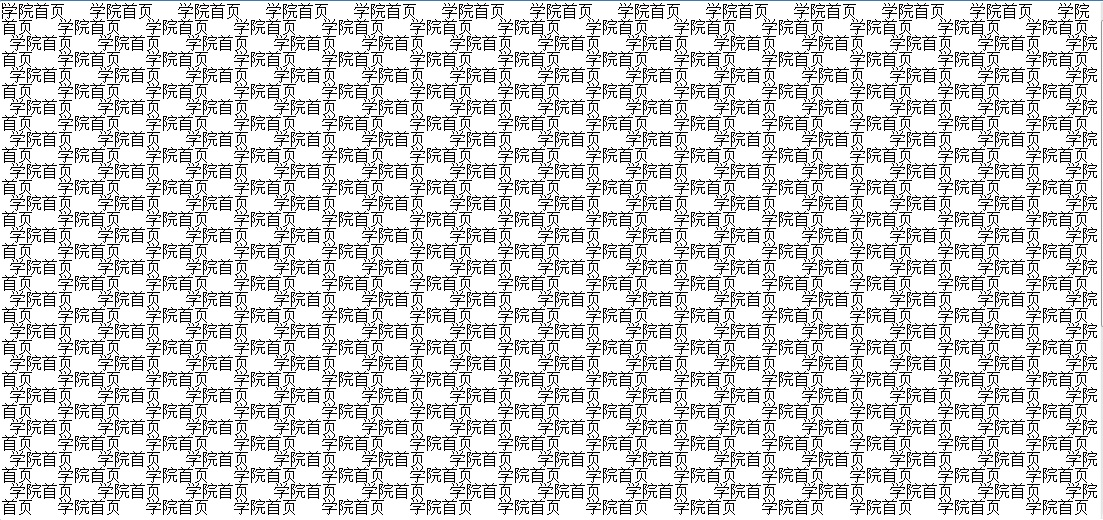
\includegraphics[width=5.00in,height=3.00in]{figure33.jpg}
\par{}
\subsection{pagerank}
我上传的pagerank文件里存储了10000+个网页的pagerank值,我们发现一个pagerank数量级为10E-5,是由于所有的pr之和为1
\subsection{site}
搜索如下
\par{}

\includegraphics[width=2.00in,height=1.00in]{28.jpg}
\par{}
结果如下
\par{}
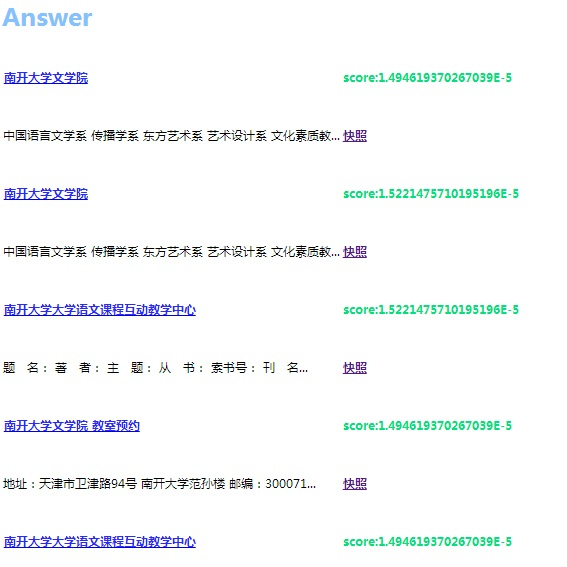
\includegraphics[width=5.00in,height=5.50in]{27.jpg}
\par{}
\subsection{filetype}
搜索如下
\par{}

\includegraphics[width=2.00in,height=1.00in]{29.jpg}
\par{}
结果如下
\par{}
得到404的结果可能是由于爬虫对pdf,doc类型的文件像html一样爬,但其实是不一样的。
\par{}
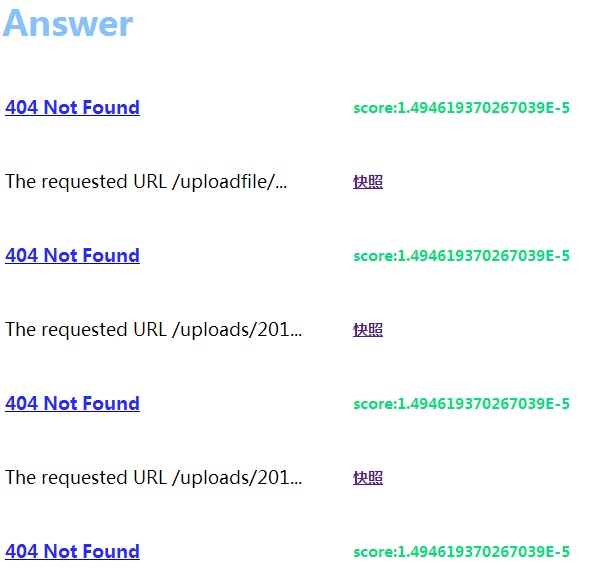
\includegraphics[width=5.00in,height=4.50in]{30.jpg}
\par{}
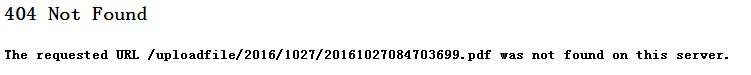
\includegraphics[width=5.00in,height=0.50in]{31.jpg}
\par{}
\subsection{短语通配}
短语在之前的"魏大鹏到数学科学学院"已经展示过来,这里仅展示通配
\par{}

\includegraphics[width=2.00in,height=1.00in]{25.jpg}
\par{}
结果如下
\par{}
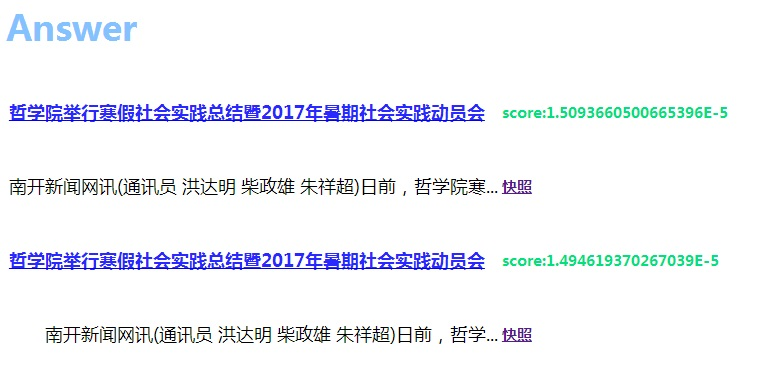
\includegraphics[width=5.00in,height=2.20in]{26.jpg}
\par{}

\includegraphics[width=5.00in,height=2.00in]{figure25.jpg}
\par{}
\subsection{查询日志}
\par{}
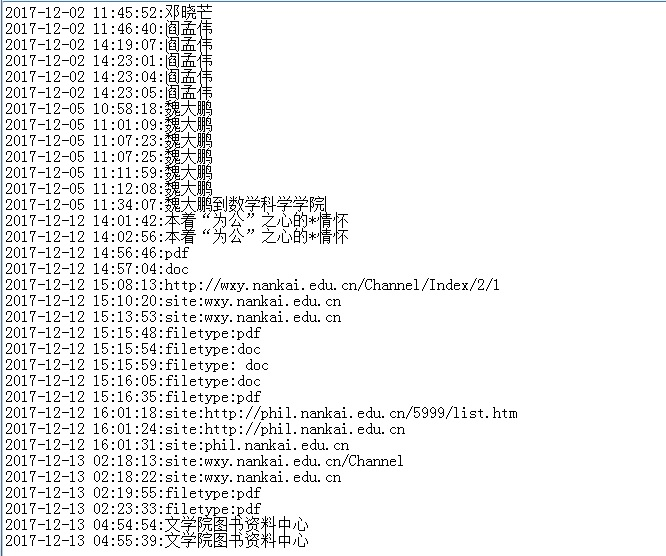
\includegraphics[width=5.00in,height=4.20in]{36.jpg}
\par{}
\subsection{网页快照}
搜索如下
\par{}

\includegraphics[width=2.00in,height=1.00in]{32.jpg}
\par{}
结果如下
\par{}
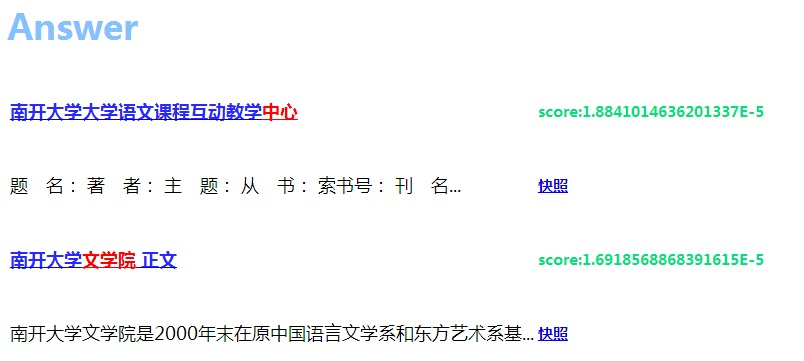
\includegraphics[width=5.00in,height=2.00in]{33.jpg}
\par{}
点击第一个的快照,结果如下
\par{}
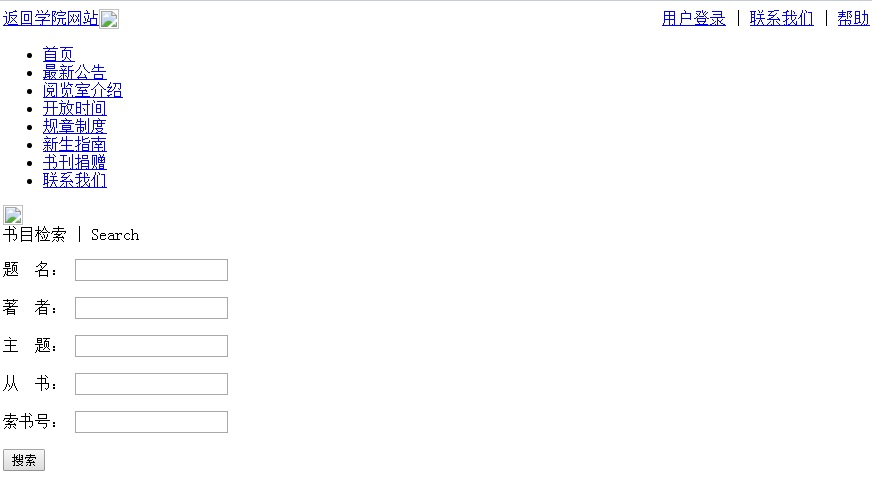
\includegraphics[width=5.00in,height=3.00in]{34.jpg}
\par{}
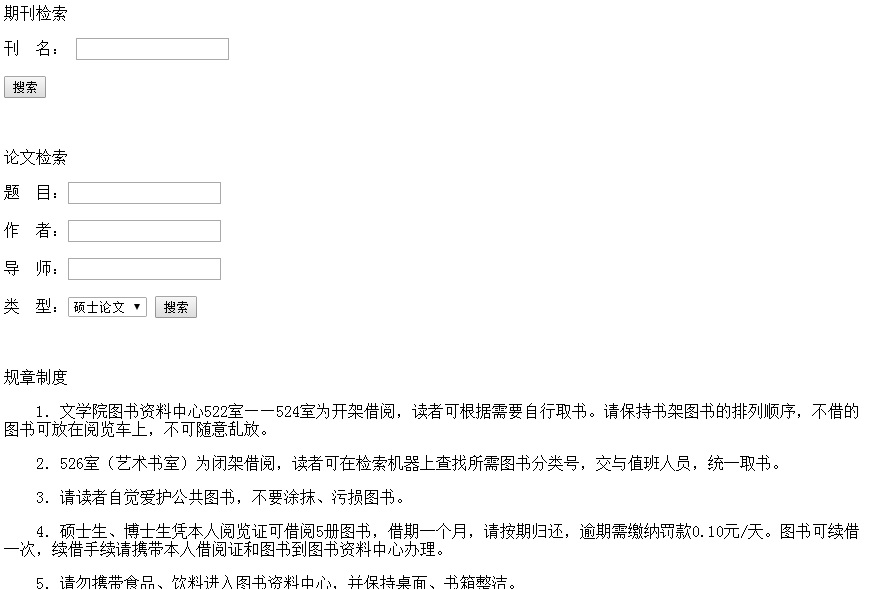
\includegraphics[width=5.00in,height=4.00in]{35.jpg}
\par{}
真实的页面如下:
\par{}
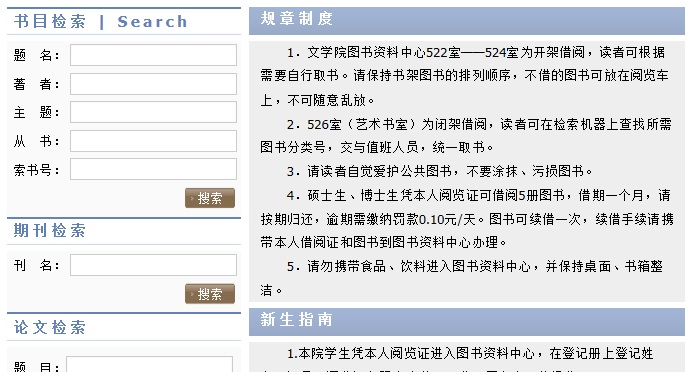
\includegraphics[width=5.00in,height=3.00in]{figure37.jpg}
\par{}
\section{设计思路及相关代码}
\subsection{WebPageSource.java文件:}
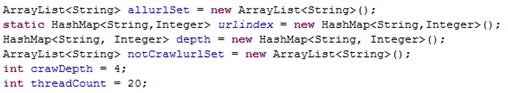
\includegraphics[width=5.00in,height=1.00in]{figure1.jpg}
    以上几个变量比较重要,其中allurlSet和notCrawlurlSet都用来存储url,区别是allurlSet会用来判断一个url是否已经包含在我们要爬或者已经爬了的url之中。而notCrawurlSet用于每次从中获取要爬的url,并且把爬了的从中remove,如果它不包含任何url(ArrayList为空)时,程序结束。
还有几个比较重要的函数,其中addUrl:
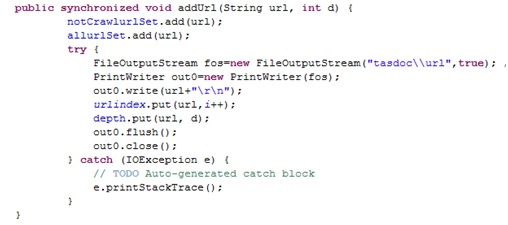
\includegraphics[width=5.00in,height=2.50in]{figure2.jpg}
    用urlindex记录url对应的id号,用d代表url距离学院官网的深度,我们限制了只爬取距离官网深度为4以内的url。还要把url加入allurlSet和notCrawlurlSet中。
\par{}
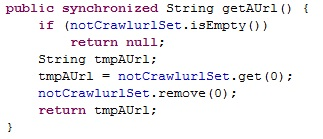
\includegraphics[width=3.00in,height=1.25in]{figure3.jpg}
\par{}
    函数getAUrl从notCrawlurlSet中获取url。
\par{}
    函数crawler():
\par{}
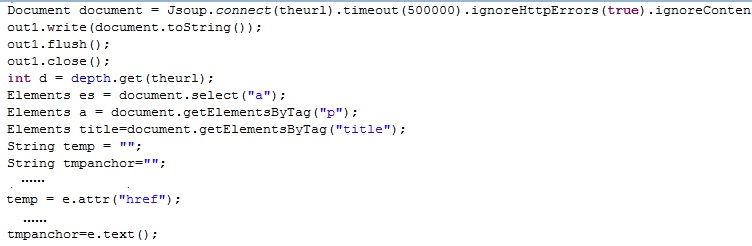
\includegraphics[width=5.00in,height=1.00in]{figure4.jpg}
\par{}
    创建document对象,根据document选取网页的标题、内容、链接以及链接对应的锚文本,同时把整个document存储到html文件夹里生成HTML文件。
接着判断链接是否符合要求,符合的话,把它加入arraylist,用于将来抓取。
\subsection{pagerank.java文件:}
\par{}
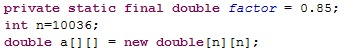
\includegraphics[width=3.00in,height=0.50in]{figure5.jpg}
\par{}
首先定义一个大小为n*n的矩阵。
接着,按照之前记录的每个网页指向的链接(id号),对矩阵进行赋值。
\par{}
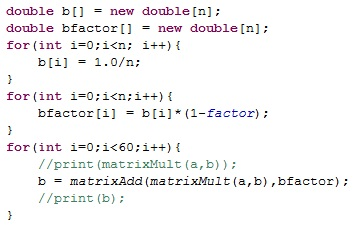
\includegraphics[width=3.20in,height=2.00in]{figure15.jpg}
\par{}
接着初始化矩阵b[n],接着构造矩阵bfactor[n]
bfactor代表以下pagerank计算公式中的(1-d)/N
\par{}
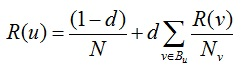
\includegraphics[width=2.00in,height=0.60in]{figure16.jpg}
\par{}
我们对初始矩阵进行60次迭代,最终矩阵会收敛,逼近每一个网页的pagerank值。
其中,用到了以下两个自定义函数。
\par{}
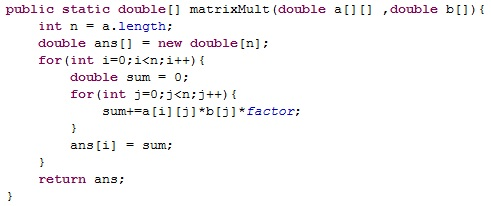
\includegraphics[width=5.00in,height=2.00in]{figure17.jpg}
\par{}
MatrixMult中的sum不断更新
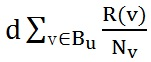
\includegraphics[width=0.50in,height=0.25in]{figure18.jpg}
而matrixAdd用于将(1-d)/N与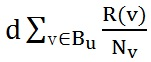
\includegraphics[width=0.50in,height=0.25in]{figure18.jpg}相加,接着把新生成的值赋予b,接着用b继续不断收敛。
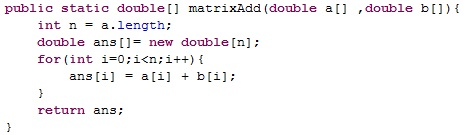
\includegraphics[width=4.50in,height=1.50in]{figure19.jpg}
\par{}
把最终经过60次迭代后收敛的矩阵b(b[0…n]的b[i]分别代表id号为i的网页的pagerank值)存储到一个文件中。
\subsection{createindex.java文件:}
用了lucene和IKAnalyzer建立索引:
\par{}
依据存储的文档,为每个document添加id,pagerank,content,name,num的值。
\par{}
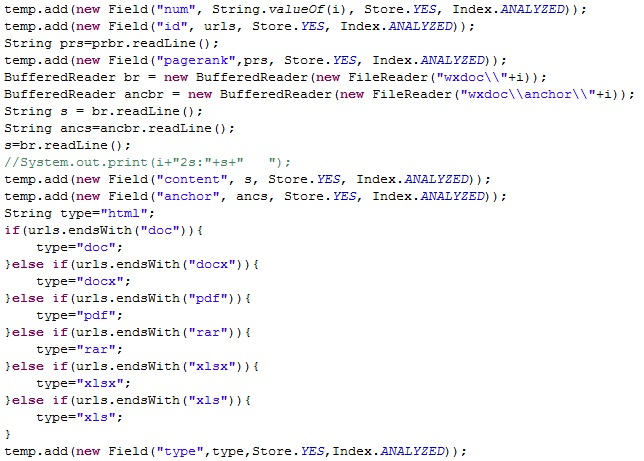
\includegraphics[width=5.00in,height=4.00in]{figure20.jpg}
\par{}
并把每个document添加到indexWriter(对应于下面的文件夹)中。
\par{}
我们生成的索引存放在indexDir文件夹里。
\par{}
在Spring tool suite中,对已创建的索引进行搜索。
\par{}
\subsection{在Filesearch.java文件中}
\par{}
    我们利用IKanalyzer以及lucene提供的IKQueryParser、IKSimilarity、QueryParser等,从索引中获取与搜索相匹配的文档。
\par{}
    接着判断是site查询,filetype查询,还是内容的查询。
\par{}
    接着获取匹配的文本中前十个文档。
\par{}
    在找到相关文档之后,对每个文档生成html文件,用于用户点击快照时显示。
\par{}
    我们知道,快照其实是搜索引擎服务器显示自己爬取了这个网页之后保存的html文件。用户查看走的是搜索引擎的流量。
\par{}
\subsection{scoredoc.java}
    在这个文件里,我们定义了一个scoredoc类,用于在jsp文件中获取每个搜索结果对应的变量值。
\par{}
    其中,getid()获取url,getcontent()获取网页内容,gettitle()获取标题,getpr()获取pagerank值,getins()获取网页简介(内容的前30字)。
\par{}
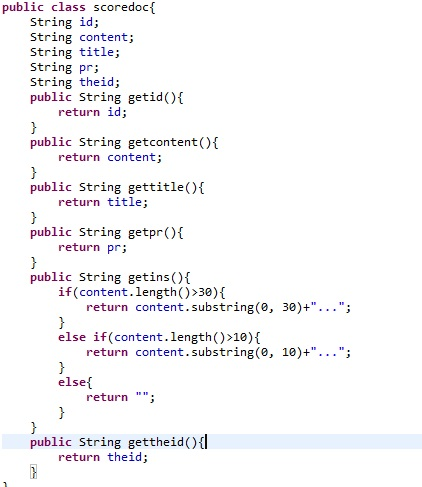
\includegraphics[width=3.00in,height=4.00in]{figure21.jpg}
\par{}
\section{相关配置}
\subsection{java文件夹}
    在\textbf{java文件夹}里src存放着java的源码。
\par{}
    其中,爬虫,计算pagerank以及建立索引是在这儿完成的,这儿的代码我都使用的相对路径。
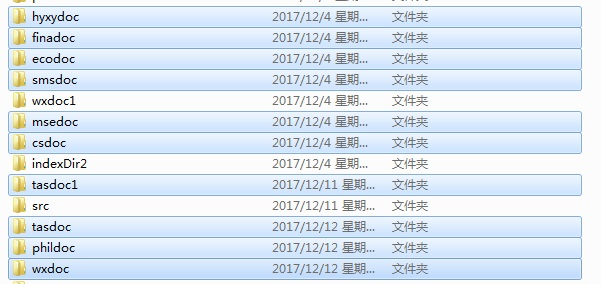
\includegraphics[width=5.00in,height=3.00in]{figure22.jpg}
    其中的phildoc代表哲学院网站网页的信息,hyxydoc代表汉语言文学院,finadoc代表金融学院,eco代表经济学院......
\par{}
    indexDir存放索引信息。
\par{}
    其中src里存放的源码,createindex用于创建索引,pagerank用于计算pr值,WebPageSource用于爬网页。
\par{}
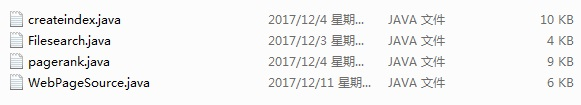
\includegraphics[width=5.00in,height=1.00in]{figure23.jpg}
\par{}
    Java程序需要引用的jar包存放在string tool suite文件夹里的"prsearch/src/main/webapp/WEB-INF/lib"里。
\par{}
\subsection{string tool suite文件夹}
    在string tool suite文件夹里存放着写成网页的源代码
\par{}
    其中"prsearch/src/main/java/com/pr/xu"文件夹里存放着后端的Java源码
\par{}
    在Filesearch.java中由于用的是绝对路径,如果要在老师那儿跑程序的话需要修改路径,分别是:
\par{}
    "private File INDEXDIR = new File("J:$\backslash\backslash$java$\backslash\backslash$WebPageSource$\backslash\backslash$indexDir"); "
\par{}
    和
\par{}
    "File writename = new File("I://html//"+i+".html");"
\par{}
    在HomeController.java中也有绝对路径老师要跑程序的话需要修改:
\par{}
    "fos = new FileOutputStream("I:$\backslash\backslash$html$\backslash\backslash$log.txt",true);"
\par{}
    文件夹"prsearch/src/main/webapp/WEB-INF/views"里存放着jsp前端源码
    在answer.jsp文件中也有绝对路径老师要跑程序的话需要修改
    href="file://localhost/J:/java/WebPageSource/wxdoc/html/"
\par{}
    在文件夹"prsearch/src/main/webapp/WEB-INF/lib"里存放着引用的jar包
\par{}
    跑网页程序时需要它们。
\section{总结}
    通过这次实验,我知道了如何写爬虫,知道了pagerank的值如何计算,以及网页之间的关联,更是熟悉了搜索引擎的实现方法。知道了运用已有的jar包实现要求的功能,知道了君子生非异也,善假于物也。也知道了如何生成日志、快照,这次实验我受益匪浅。
\end{flushleft}
\end{document}
